\begin{pa} \label{PA:7.6} Recall that one model for population growth states that a population grows at a rate proportional to its size.

  \ba
\item We begin with the differential equation 
  $$
  \frac{dP}{dt} = \frac12 P.
  $$
  Sketch a slope field below as well as a few typical solutions on the axes provided.

  \begin{center}
    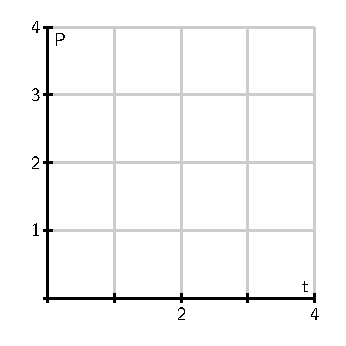
\includegraphics{figures/7_6_preview.eps}
  \end{center}

\item Find all equilibrium solutions of the equation $\frac{dP}{dt} = \frac12 P$ and classify them as stable or
  unstable.  

\item If $P(0)$ is positive, describe the long-term behavior of the
  solution to $\frac{dP}{dt} = \frac12 P$.  
\item Let's now consider a modified differential equation given by
  $$
  \frac{dP}{dt} = \frac 12 P(3-P).
  $$
  As before, sketch a slope field as well as a few typical solutions on the following axes provided.
  \begin{center}
    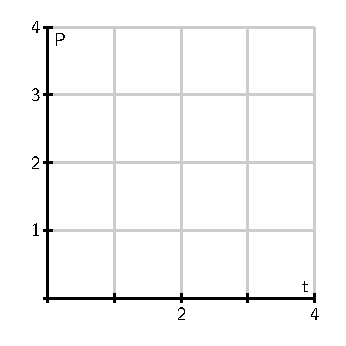
\includegraphics{figures/7_6_preview.eps}
  \end{center}

\item Find any equilibrium solutions and classify them as stable or
  unstable.  

\item If $P(0)$ is positive, describe the long-term behavior of the
  solution.  

\ea
\end{pa} 
\afterpa
